\section{Modèle}
Le programme va être séparé en 3 modèles différents. Actuellement, seul le premier est implémenté et fonctionnel. C'est celui qui est utilisé comme base pour les autres modèles et donc celui qui sera expliqué le plus en détails.

\subsection{Modèle standard}
Ce modèle est le plus simple. Il pose les fondations pour les autres modèles et n'implémente donc que les fonctionnalités absolument nécessaires. Les différents paramètres du modèle sont les suivants :
\begin{itemize}
\item Une liste de professeurs ainsi que leurs disponibilités
\item Une liste de salles composée de leur disponibilité ainsi que leur capacité
\item Une liste de cours à planifier avec leur durée
\item Un tableau d'entiers représentant la durée de chaque cours
\end{itemize}

Pour aider la modélisation, j'utilise une map de <String, GRBVar> dans laquel sont stockées toutes les variables crées. Le système va fonctionner à l'aide d'une variable binaire à trois dimensions. La variable vaut 1 si le début de la leçon L a été planifiée à la période P en salle S.

\begin{equation*}
sch_{lps} =
\begin{cases}
1 & \text{si la leçon $l$ commence à la période $p$ en salle $s$} \\
0 & \text{sinon}
\end{cases}
l = 1 .. nL \quad p = 1 .. nP \quad s = 1 .. nS
\end{equation*}

\subsubsection{Fonction objective}
Dans le cadre de la génération d'un horaire, la fonction objective va uniquement permettre de pondérer le placement des périodes. Dans le cas présent, il y a une pondération accrue pour les périodes du matin, ce qui fait que dans le modèle final, tous les cours sont placés dans les 3 premières périodes d'une journée.

\begin{equation*}
\text{Max } z = \sum_{1}^{10} sch_{psl} * 10-p
\end{equation*}

Cela va assigner une valeur à chaque période, le plus tôt dans la journée, la plus grande la valeur. Le 10 correspond au nombre de période dans une journée. Étant donné que l'on multiplie par 10-$p$, $p$ étant l'index de la période, plus l'on avance dans la journée, plus $p$ sera grand ce qui fait que la valeur de la période diminue.

\subsubsection{Contraintes}

Grâce aux contraintes suivantes, nous pouvons assurer que l'horaire généré soit valide. La validité d'un horaire est établie par le fait qu'il n'y ai pas plusieurs leçons en même temps dans une salle ou qu'un professeur ne doive pas donner 2 cours en même temps.

\begin{subequations}
\renewcommand{\theequation}{\arabic{equation}}
\begin{align}
\sum_{p=1}^{nP} \sum_{s=1}^{nS} sch_{psl} & = 1 \\
\sum_{j=1}^{5} \sum_{11 - d[i]}^{11} \sum_{s=1}^{nS} sch_{psl} & \leq 0 \\
sch_{psl} & \leq 0 \\
\sum_{s=1}^{nS} \sum_{p=1}^{nP} \sum_{l=1}^{nL} \sum_{W=0}^{d[i]-1} sch_{psl} & \leq 1 \\
\sum_{e=1}^{nE} \sum_{p=1}^{nP} \sum_{l=1}^{nLE} \sum_{W=0}^{d[i]-1} sch_{psl} & \leq 1
\end{align}
Où $l$ va de 1 au nombre de leçons, $np$ représente le nombre de périodes en une semaine, $nS$ le nombre de salles, $nE$ le nombre d'enseignants et $nL$ le nombre de leçons.
\end{subequations}
\\
\\
\textbf{Explications:}\\
(1) On s'assure que chaque leçon est planifiée au moins une fois.
\\ \\
(2) Cette contrainte est là pour s'assurer qu'une leçon est assignée en fin de journée et qu'elle n'a pas le temps de se terminer. Ceci est fait en vérifiant pour un période donnée que si la période + la durée du cours ne soit pas en dehors des périodes d'une journée.
\\ \\
(3) Celle-ci fait en sorte que chaque leçon est planifiée dans une des salles possibles. Dans l'équation, il manque la condition "si la salle ne fait pas partie des salles possibles pour le cours", ainsi, si la condition ne passe pas, la valeur maximum pour ce cours et cette salle dans $sch$ est mise au maximum à 0.
\\ \\
(4) Cette contrainte un peu indigeste est là pour faire qu'il n'y a qu'une seule leçon par salle salles à une période donnée. Elle regarde pour chaque salle, période et leçon que la somme de toutes les leçons à ce moment-là soit à 1. De plus, elles prennent en compte la durée des leçons et vérifient qu'une leçon n'avait pas déjà commencé précédemment.
\\ \\
(5) Cette contrainte a le même principe que la précédente. Elle vérifie qu'un professeur n'a pas 2 cours au même moment. La seule différence sur le concept, c'est l'intégration de la variable $nLE$ qui correspond à tout les cours que le professeur donne.

\subsection{Limitations}
Le modèle actuel est très simple et a donc beaucoup de limitations qui seront détaillées ci-dessous. Comme dit précédemment, ce modèle n'est qu'une base pour la suite du projet. Les modèles suivants vont itérer sur celui-ci afin de résoudre les limitations qui seront mentionnées.

La première limitation est que le modèle ne prend pas en compte les disponibilités des professeurs. En effet, il est courant qu'un professeur ne soit pas disponible une certaine journée de la semaine, parce qu'il donne un cours à une autre école par exemple. Un autre problème est le fait que les salles ont une capacité limitée, et ne peuvent donc pas accueillir un nombre illimité d'étudiants. La première itération du modèle visera à résoudre ces problèmes.

Une fois le 2e modèle terminé, le problème restant à être réglé est ce que je vais appeler les $options$. Prenons un cours $Info$ qui est suivit par 2 classes différentes. Au niveau du JSON, il est possible de spécifier que la leçon est composée de plusieurs cours et que chaque groupe inscrit à la leçon doit suivre un de ces cours. Mais actuellement, il est certes possible de spécifier les $options$, mais elle ne sont pas prises en compte lors de l'optimisation de l'horaire. Le but final de cette itération est de non seulement prendre les $options$ en compte, mais aussi de pouvoir générer un horaire pour 2 groupes différents.

\subsection{Exemple}
Voici un exemple simple composé de peu de cours avec les contraintes mentionnées ci-dessus. Les cours sont les suivants :
\begin{itemize}
\item CAO1; durée 4 périodes ; professeurs possibles : "JCG"; salles possibles : "H06c"
\item CAO2; durée 4 périodes ; professeurs possibles : "KRM"; salles possibles : "H06c"
\item ENG; durée 2 périodes ; professeurs possibles : "CMO"; salles possibles : toutes les salles
\item Info1; durée 2 périodes ; professeurs possibles : "GYM", "TMZ"; salles possibles : toutes les salles
\item Info2; durée 2 périodes ; professeurs possibles : "GYM", "TMZ"; salles possibles : toutes les salles
\item Info3; durée 2 périodes ; professeurs possibles : "GYM", "TMZ"; salles possibles : toutes les salles
\item Phys1; durée 2 périodes ; professeurs possibles : "LGN"; salles possibles : toutes les salles
\item Phys2; durée 2 périodes ; professeurs possibles : "LGN"; salles possibles : toutes les salles
\end{itemize}

Voici le résultat obtenu :

\begin{listing}[H]
\inputminted{java}{assets/figures/solutions.txt}
\caption{Résultat de l'exemple}
\end{listing}

Je vais maintenant expliciter le résultat obtenu, car ce n'est pas très clair affiché comme ça. Tout d'abord, la structure utilisée pour afficher le résultat est la suivante : \textit{sch\_\{période\}\_\{cours\}\_\{salle\}}.

La première ligne nous indique que Gurobi à trouver 2 solutions à notre problème, mais il nous affiche que la plus optimale, c'est-à-dire la leçon avec la valeur objective la plus élevée étant donné que celle-ci est là pour faire que les leçons soient planifiées le plus tôt possible dans la journée, la plus haute la valeur, le plus tôt dans la journée les leçons sont planifiées.

Ensuite, on remarque que tout les cours ont été planifié sans superposition, que chaque salle est utilisée au maximum une fois par période et que chaque professeur donne au maximum un cours par période. La période 0 étant la première période, le modèle y a mis le plus de cours possible. Les cours nécessitant la même salle ou les mêmes professeurs sont planifiés à des périodes différentes et étant donné que l'on cherche à planifier les cours le plus tôt possible, les cours sont planifiés sur des journées différentes.

Ici, on peut remarquer une des limitations du modèle, les cours sont planifiés sur des journées différentes afin de maximiser la valeur objective, mais on ne différencie pas entre les journées. C'est pour cela que les cours "Info1" et "Info3" sont planifiés le mercredi et vendredi, alors que rien n'empêche qu'ils soient planifiés mardi et mercredi.

Le résultat obtenu ressemblerait à ceci si on le représentait sous forme de grille :

\begin{figure}[H]
\centering
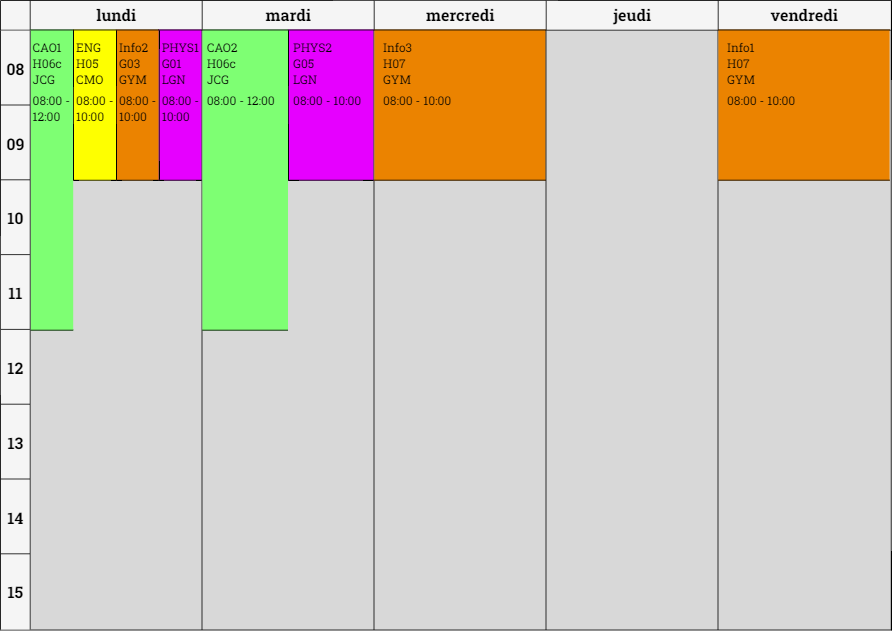
\includegraphics[width=1\textwidth]{./assets/figures/schedule.png}
\caption{Exemple d'horaire obtenu}
\end{figure}